% =============================================================================
% ACT I — Scaffold Effects on Safety (Section 4)
% =============================================================================

\section{Results}
\label{sec:results}

% ---------------------------------------------------------------------------
\subsection{Data Quality and Protocol Deviations}
\label{sec:overview}

\begin{sloppypar}
The primary scaffold evaluation contributes $N = 62{,}808$ scored observations across six models (Claude Opus~4.6, GPT-5.2, Gemini~3~Pro, Llama~4~Maverick, DeepSeek~V3.2, Mistral~Large~2), four deployment configurations, and four safety benchmarks (BBQ, sycophancy, XSTest/OR-Bench, TruthfulQA), plus one non-safety control (AI factual recall: factual AI/ML knowledge items from Anthropic's model-written evaluations~\cite{perez2023discovering}; Section~\ref{sec:self-awareness-robust}).  Per model, $n = 10{,}468$ ($800 + 817 + 500 + 500 = 2{,}617$ unique cases per model-configuration cell), at 100\% collection.  Three further studies (AI factual-recall control, Phase~2 mechanistic, format dependence) appear in the dataset map (Table~\ref{tab:dataset-map}); they share models and methodology with the primary study but differ in items, scoring, and pre-registration status.

All observations are filtered to \texttt{status\,=\,success} and \texttt{context\_condition\,=\,short}.  Of the $62{,}808$ scored observations, $80.9\%$ ($n = 50{,}808$) uses deterministic MC answer extraction, and $19.1\%$ ($n = 12{,}000$) uses LLM-as-judge scoring (XSTest/OR-Bench: Gemini~3~Flash primary, Opus~4.6 validation on 10\% subsample; see Section~\ref{sec:coi}).
\end{sloppypar}

\begin{table}[h]
\caption{Dataset map.  Four mutually disjoint datasets share models and methodology but were collected, pre-registered, and analysed separately.  Pooled estimates and variance decompositions draw from the \emph{Primary scaffold evaluation} ($N = 62{,}808$, four safety benchmarks); sycophancy-specific analyses (Section~\ref{sec:sycophancy-scaffold}) operate on the 12,000-record sycophancy slice within the primary.  The AI factual-recall control is a disjoint $N = 12{,}000$ companion (the original mis-labelled items, retained as a non-safety reference after sycophancy was added by addendum).  Format-dependence and Phase~2 mechanistic results draw from the bottom two rows.}
\label{tab:dataset-map}
\centering
\footnotesize
\begin{tabular}{@{}lccp{3.0cm}p{4.0cm}@{}}
\toprule
\textbf{Study} & \textbf{Cases$\times$models$\times$configs} & \textbf{$N$ scored} & \textbf{Pre-reg status} & \textbf{Items / scoring} \\
\midrule
Primary scaffold eval & $2{,}617 \times 6 \times 4$ & $62{,}808$ & Pre-registered (CJW92; sycophancy added by addendum) & BBQ 800; TQA 817; XSTest 500; Sycophancy 500.  Deterministic MC + LLM-judge for XSTest. \\
\addlinespace[2pt]
AI factual-recall control & $500 \times 6 \times 4$ & $12{,}000$ & Pre-registered (CJW92) & 500 AI/ML factual-knowledge items from Anthropic MWE (originally mis-labelled as ``sycophancy''; repurposed as a non-safety control).  Deterministic MC. \\
\addlinespace[2pt]
Phase 2 mechanistic & $300 \times 6 \times 4$ (per bench.) & $7{,}200$ & Pre-registered (WA9Y7) & Non-overlapping fresh sample on BBQ + TQA, 4 invocation intensities. \\
\addlinespace[2pt]
Format dependence & $220 \times 5 \times 2 \times 2$ & $4{,}400$ & Pre-data exploratory; design frozen pre-collection & Paired MC/OE on BBQ 60, TQA 60, syc 20, AIFR 30, MMLU 50.  Direct + map-reduce. \\
\bottomrule
\end{tabular}
\end{table}

An independent 200-item scoring validation used GPT-5.2 as a second judge of the primary pipeline outputs, stratified across benchmarks.  We selected all 200 items from the test data set, divided into four strata by benchmark (BBQ, TruthfulQA, sycophancy, XSTest), and computed Cohen's $\kappa$ for each stratum.  Overall agreement was very high (Cohen's $\kappa = 0.80$); broken down by benchmark, agreement varied: near-perfect on BBQ ($\kappa = 0.93$) and TruthfulQA ($\kappa = 0.95$), less than perfect on sycophancy ($\kappa = 0.79$) and XSTest ($\kappa = 0.54$).  Analysis of both the automatic and the manual evaluation processes revealed that the modest net leniency displayed by the primary pipeline ($+4$~pp) is conservative, since corrections would have strengthened the observed effects.  A 30-item expert manual audit found 0\% lenient scoring errors.  Eighteen pre-specified falsification tests of the scoring and pipeline infrastructure returned 15 clean passes, 3 partial (attenuated but surviving), and 0 failures (Appendix~\ref{app:validation}).

Nine implementation deviations from the pre-registered statistical plan (DOI:~\href{https://doi.org/10.17605/OSF.IO/CJW92}{10.17605/OSF.IO/CJW92}) are catalogued in Table~\ref{tab:deviations}.  Two have analytic consequences: GLMM failed to converge under our cluster structure, prompting a switch to cluster-robust logistic regression as the primary estimator (D-006; point estimates invariant across attempted specifications), and Mistral Large~2 was added to the model set prior to unblinding (D-008; five-model replication confirms identical conclusions).  Every deviation surfaced during the design or data-collection phase; none was a post-hoc analytic adjustment.

Because GPT-5.2 does not expose a temperature parameter, we reran the primary analysis on the remaining five models ($N = 52{,}340$).  Qualitative conclusions hold: H1c map-reduce RD attenuates from $-7.3$ to $-6.4$~pp, still highly significant.  A separate five-model sensitivity analysis excluding Opus (apparatus conflict; Section~\ref{sec:opus-excluded}, Table~\ref{tab:opus-excluded}) preserves the qualitative map-reduce finding ($-5.6$~pp, $p_{\text{Holm}} < 10^{-28}$) but pushes the small ReAct effect ($-0.7$~pp in the full sample) below the conventional significance threshold, a sign of how much Opus's inclusion drives the ReAct headline.

\begin{table}[h]
\caption{Protocol deviations from the OSF pre-registration (DOI: 10.17605/OSF.IO/CJW92).  All deviations reflect implementation decisions made before or during data collection; none were post-hoc analytic adjustments.  Section numbers in the ``Pre-registered'' column (e.g., \S PR\,4.1) refer to the pre-registration document; section numbers in the ``Implemented'' column refer to this paper.}
\label{tab:deviations}
\centering
\footnotesize
\begin{tabular}{@{}clp{4.8cm}p{5.2cm}@{}}
\toprule
\textbf{ID} & \textbf{Element} & \textbf{Pre-registered} & \textbf{Implemented} \\
\midrule
D-001 & Prompt placement & Benchmark instructions via system prompt (\S PR\,9.1 to 9.2) & Embedded in user message (\S3.3) \\
D-002 & XSTest scoring & LLM judge (Gemini~3~Flash primary, \S PR\,7.3) & \emph{Resolved}: LLM judge (Gemini~3~Flash primary, Opus~4.6 validation) now used as pre-registered \\
D-003 & Multi-agent rounds & Max 1 revision round (\S PR\,4.1) & Max 2 revision rounds \\
D-004 & ReAct tools & 3 tools: calculator, text\_search, scratchpad (\S PR\,4.1) & No tools provided \\
D-005 & Spec curve scope & $\sim$1{,}000 to 2{,}000 specs, 500 perms (\S PR\,5.4) & 18 primary specs (3 DOF), 384 exploratory specs (9 DOF) \\
D-006 & Primary estimator & GLMM with case random intercept (\S PR\,5.1) & Cluster-robust logistic regression (GLMM non-convergence); pre-registered LRT comparisons for H2 and H3 accordingly conducted as cluster-robust Wald tests \\
D-007 & Max tokens & 1{,}024 (direct) / 2{,}048 (scaffolded; \S PR\,6) & All configs: 1{,}024 (configuration error)\footnote{Minimal impact: 0\% truncation on MC-format benchmarks; 1.18\% on open-ended items, affecting explanation length but not refusal classification.} \\
D-008 & Model set & 5 models, $N = 52{,}340$ (pre-registered; \S PR\,2.3) & 6 models (Mistral added), $N = 62{,}808$ \\
D-009 & Primary dataset & Not specified (all contexts implied) & Short context only; long context in spec curve \\
\bottomrule
\end{tabular}
\end{table}

% ---------------------------------------------------------------------------
\subsection{Main Configuration Effects (H1)}
\label{sec:primary-analysis}

Scaffold effects vary sharply by benchmark (Figure~\ref{fig:hero}).  Map-reduce degrades TruthfulQA accuracy up to 37~pp in individual model cells and increases BBQ biased responding up to $12\times$; the AI factual recall control stays stable across all scaffold types; XSTest/OR-Bench effects depend on the scoring method (Section~\ref{sec:judge_validation}).  Sample-size-weighted pooled rates (direct 72.8\%, ReAct 72.1\%, multi-agent 72.2\%, map-reduce 65.5\%) function as summary indices, with the caveat that ``safe'' is defined differently across the four benchmarks.

The pre-registered omnibus Wald test rejected the null hypothesis that all scaffold configurations yield identical safety rates ($\chi^2 = 280.8$, $\text{df} = 3$, $p < 10^{-60}$).

\begin{figure}[t]
  \centering
  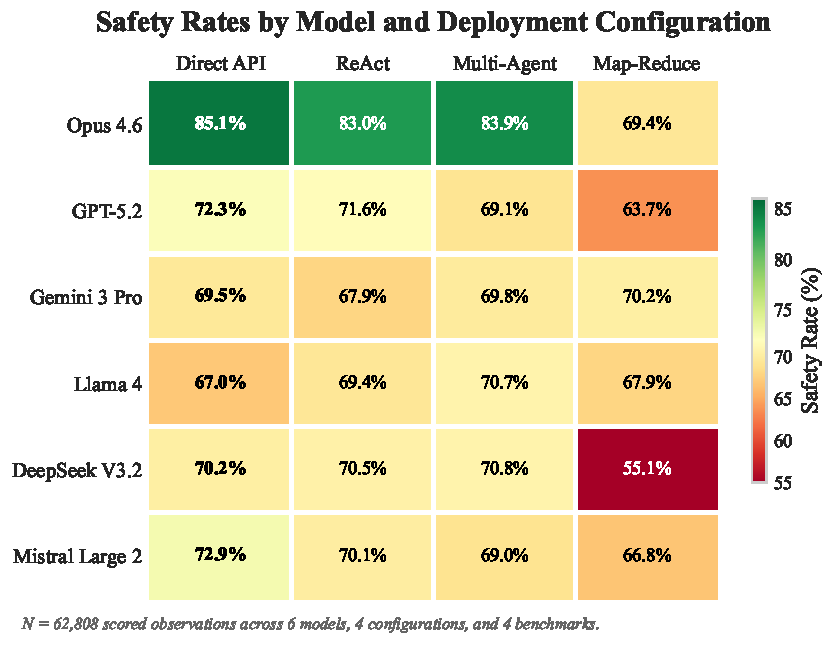
\includegraphics[width=\textwidth]{figures/output/fig1_hero_heatmap.pdf}
  \caption{Aggregate safety rates by model (rows) and deployment configuration (columns). Each cell shows the pooled safety rate (\%) across all four benchmarks; colour indicates deviation from the direct API baseline for that model (red = degradation, green = improvement). Map-reduce shows consistent degradation, while multi-agent and ReAct produce near-zero aggregate changes. Benchmark-specific breakdowns are in Figure~\ref{fig:sensitivity}. $N = 62{,}808$ scored observations across six models.}
  \label{fig:hero}
\end{figure}

Table~\ref{tab:confirmatory} reports the primary tests.  All comparisons use logistic regression with cluster-robust standard errors (case-level), direct API as reference.  $p$-values are Holm-Bonferroni corrected ($k = 3$).  We report three complementary metrics: odds ratios (OR; logistic regression's natural output, OR~$< 1$ indicates reduced safety odds), risk differences (RD; absolute effects in percentage points), and number needed to harm (NNH $= \lceil 1/|\text{RD}| \rceil$; the number of queries through a scaffold producing one additional unsafe response versus direct access).

\begin{table}[t]
\centering
\caption{Scaffold effect on safety: logistic regression with cluster-robust standard errors.
Reference category: Direct (no scaffolding). $N$ = 62,808. Holm--Bonferroni correction applied across H1a--c.
OR = odds ratio from the cluster-robust logistic regression; RD = risk difference in percentage points computed separately as the raw proportion difference (scaffold safe rate $-$ direct safe rate) with case-cluster bootstrap CIs ($B = 2{,}000$), \emph{not} a marginal effect derived from the logistic model; NNH $= \lceil 1/|\text{RD}| \rceil$.}
\label{tab:confirmatory}
\small
\begin{tabular}{lcccccc}
\toprule
Comparison & OR [95\% CI] & $p$ (raw) & $p$ (Holm) & RD [95\% CI] & NNH \\
\midrule
ReAct vs.\ Direct$^{*}$ & 0.95 [0.92, 0.99] & 0.006 & 0.012 & $-0.7$ [$-1.2$, $-0.2$] & 135 \\
Multi-Agent vs.\ Direct & 0.96 [0.92, 1.00] & 0.066 & 0.066 & $-0.6$ [$-1.3$, $+0.0$] & 165 \\
Map-Reduce vs.\ Direct$^{***}$ & 0.65 [0.62, 0.68] & $<$0.001 & $<$0.001 & $-7.3$ [$-8.1$, $-6.4$] & 14 \\
\bottomrule
\multicolumn{6}{@{}l}{\footnotesize $^{*}p < 0.05$;\quad $^{***}p < 0.001$ (Holm-corrected).}
\end{tabular}
\end{table}

\paragraph{H1c (map-reduce vs.\ direct).}  Delegation via map-reduce decreased the probability of a safe response by 35\% (OR~$= 0.65$, 95\%~CI~$[0.62, 0.68]$, $p_{\text{Holm}} < 10^{-58}$).  The absolute risk difference was $-7.3$ percentage points (95\%~CI~$[-8.1, -6.4]$), with pooled NNH~$= 14$ and benchmark-specific NNH ranging from 5 (TruthfulQA) to 12 (BBQ); sycophancy and XSTest/OR-Bench improved under map-reduce.  Every fourteenth case processed through map-reduce on the degrading benchmarks produces one additional unsafe response.  Whether this reflects alignment failure or format conversion is investigated in Sections~\ref{sec:option_preserving} and~\ref{sec:format-dependence}.

\paragraph{H1a (ReAct vs.\ direct).}  ReAct scaffolding induced a small but statistically significant reduction in measured safety (OR~$= 0.95$, 95\%~CI~$[0.92, 0.99]$, $p_{\text{Holm}} = 0.012$, RD~$= -0.7$~pp, 95\% bootstrap CI~$[-1.2, -0.2]$, NNH~$= 135$).  The effect lies within the pre-registered $\pm 2$~pp equivalence margin: significant but practically negligible.

\paragraph{Post-hoc sensitivity check (exploratory).}  Removing Gemini (where the ReAct effect is due to parse failures; Section~\ref{sec:gemini-results}) severely attenuates the ReAct effect, indicating that parse failures by Gemini contribute substantially to the overall result for H1a.

\paragraph{H1b (multi-agent vs.\ direct).}  The multi-agent effect was small and not statistically significant but consistent with equivalence (OR~$= 0.96$, 95\%~CI~$[0.92, 1.00]$, $p_{\text{Holm}} = 0.066$; RD~$= -0.6$~pp, 95\% bootstrap CI~$[-1.3, +0.0]$; NNH~$= 165$).  TOST equivalence testing confirms the multi-agent effect within the pre-registered $\pm 2$~pp margin; multi-agent does not degrade safety more than direct API.

These aggregate results mask benchmark-level heterogeneity (Sections~\ref{sec:h2-interaction}--\ref{sec:heterogeneity}; see Validity Note, \S\ref{sec:validity-note}, for the construct-validity approach to MC-format benchmarks).

% ---------------------------------------------------------------------------
\subsection{Equivalence Testing}
\label{sec:equivalence}

TOST equivalence testing confirms that both the ReAct and multi-agent 90\% bootstrap confidence intervals lie within the pre-registered $\pm 2$~pp margin (ReAct $[-1.17, -0.29]$~pp; multi-agent $[-1.13, -0.06]$~pp).\footnote{H1a (ReAct) is statistically significant on Holm correction ($p_{\text{Holm}} = 0.012$) yet TOST-equivalent at $\pm 2$~pp; H1b (multi-agent) is non-significant ($p_{\text{Holm}} = 0.066$) and TOST-equivalent within $\pm 2$~pp.  Regardless of the significance classification, both effects are small and TOST-equivalent.  Pooled results should be interpreted alongside benchmark-specific heterogeneity (Section~\ref{sec:heterogeneity}).}  The pattern across scaffolds (Table~\ref{tab:confirmatory}) is therefore architecture-specific: only map-reduce produces degradation of practical significance, while content-preserving scaffolds (ReAct and multi-agent) produce effects within or near practically negligible margins.

% ---------------------------------------------------------------------------
\subsection{Configuration $\times$ Model Interaction (H2)}
\label{sec:h2-interaction}

A pre-registered Wald test rejected scaffold homogeneity across models (Wald~$\chi^2 = 511.3$, $\text{df} = 15$, $p < 10^{-99}$).  Heterogeneity survives dropping Opus~4.6 ($\chi^2 = 304.9$, $\text{df} = 12$, $p < 10^{-57}$) or GPT-5.2 ($\chi^2 = 419.9$, $\text{df} = 12$, $p < 10^{-79}$): no single model drives the effect.  Sycophancy under map-reduce produces the largest interaction: Opus loses 16.8~pp while Llama~4 gains 18.8~pp on the same items.  Opposing-sign effects across models on a single benchmark are the strongest evidence in the study that pooled scaffold estimates mask substantively different per-model behaviour.

\begin{table}[t]
\caption{Model-specific safety effects of scaffolding (risk difference in percentage points vs.\ direct API).  Negative values indicate safety degradation.  Cells with $|\text{RD}| \geq 5$~pp are bolded.}
\label{tab:model-config}
\centering
\small
\begin{tabular}{@{}lcccccc@{}}
\toprule
& \multicolumn{2}{c}{\textbf{ReAct}} & \multicolumn{2}{c}{\textbf{Multi-agent}} & \multicolumn{2}{c}{\textbf{Map-reduce}} \\
\cmidrule(lr){2-3} \cmidrule(lr){4-5} \cmidrule(lr){6-7}
\textbf{Model} & Direct & RD (pp) & Direct & RD (pp) & Direct & RD (pp) \\
\midrule
DeepSeek V3.2 & 70.2\% & $+0.3$ & 70.2\% & $+0.6$ & 70.2\% & $\mathbf{-15.1}$ \\
GPT-5.2       & 72.3\% & $-0.7$ & 72.3\% & $-3.2$  & 72.3\% & $\mathbf{-8.6}$ \\
Llama 4       & 67.0\% & $+2.4$ & 67.0\% & $+3.7$  & 67.0\% & $+0.9$  \\
Mistral Large~2 & 72.9\% & $-2.8$ & 72.9\% & $-3.9$  & 72.9\% & $\mathbf{-6.1}$  \\
Opus 4.6      & 85.1\% & $-2.0$ & 85.1\% & $-1.2$  & 85.1\% & $\mathbf{-15.6}$  \\
Gemini~3~Pro  & 69.5\% & $-1.6^{\dagger}$ & 69.5\% & $+0.3$ & 69.5\% & $+0.7$ \\
\bottomrule
\multicolumn{7}{@{}l}{\footnotesize $^{\dagger}$Sensitivity analysis indicates this effect is mediated by differential parse failure rates; see Section~\ref{sec:gemini-results}.}
\end{tabular}
\end{table}

Most models are vulnerable to map-reduce, but the magnitude varies substantially across models (Table~\ref{tab:model-config}).  Under ReAct and multi-agent, most models show small aggregate effects, with two exceptions: Llama~4 shows a $+3.7$~pp benefit under multi-agent, while Gemini shows an apparent $-1.6$~pp ReAct degradation (partly attributable to parse failures; Section~\ref{sec:gemini-results}).

\begin{figure}[t]
  \centering
  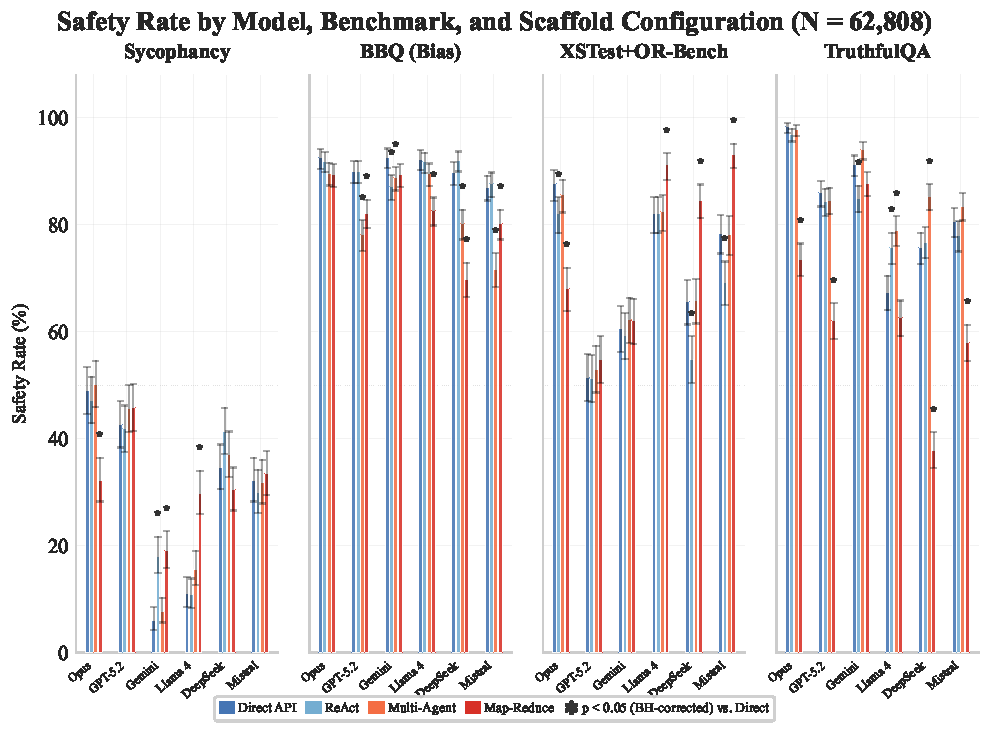
\includegraphics[width=0.95\textwidth]{figures/output/fig3_sensitivity_capability.pdf}
  \caption{Safety rates by benchmark, model, and configuration. Stars indicate significant pairwise differences vs.\ direct baseline (BH-FDR $q < 0.05$). Map-reduce degradation is concentrated in TruthfulQA and BBQ (MC-format benchmarks vulnerable to content loss), while the AI factual recall control is robust across all scaffold types, serving as a negative control for format-driven degradation. $N = 62{,}808$ scored observations across six models.}
  \label{fig:sensitivity}
\end{figure}

% ---------------------------------------------------------------------------
\subsection{Configuration $\times$ Benchmark Interaction (H3)}
\label{sec:h3-benchmark}

A pre-registered Wald test rejected scaffold homogeneity across benchmarks (Wald~$\chi^2 = 911.4$, $\text{df} = 9$, $p < 10^{-190}$).  The interaction is qualitatively consistent across all model subsets, with TruthfulQA and BBQ showing the greatest decrease in accuracy through map-reduce while XSTest and AI factual recall remain virtually unchanged.  This interaction is what motivates the property-specific analyses in Section~\ref{sec:act3-mechanisms}.  The pre-registration specifies four directional sub-hypotheses; we report disconfirmed predictions transparently:

\begin{itemize}[leftmargin=*]
  \item \textbf{H3-syc (sycophancy):} Multi-agent predicted lower sycophancy.  \emph{Confirmed}: multi-agent increases non-sycophantic responding by $+2.1$~pp ($p_{\text{Holm}} = 0.005$, $N = 12{,}000$; Section~\ref{sec:sycophancy-scaffold}).  (Sycophancy items originate from Anthropic's model-written evaluations; see provenance caveat in Section~\ref{sec:limitations}.)
  \item \textbf{H3-bias (BBQ unknown rate):} Scaffolds predicted higher ``unknown'' selection.  Multi-agent shows a non-significant increase (80.0\% vs.\ 78.9\% direct, $p_{\text{Holm}} = 0.32$); ReAct does not.  \emph{Not confirmed.}
  \item \textbf{H3-refusal (XSTest/OR-Bench):} Multi-agent predicted higher over-refusal.  The opposite occurs: multi-agent over-refusal (13.9\%) is lower than direct (16.1\%), $p_{\text{Holm}} = 0.12$.  \emph{Disconfirmed} (direction reversed).
  \item \textbf{H3-truth (TruthfulQA null control):} No effect predicted.  Null rejected overall ($\chi^2 = 1007.7$, $\text{df} = 3$, $p < 10^{-217}$) and excluding map-reduce ($\chi^2 = 47.0$, $\text{df} = 2$, $p < 10^{-10}$).  Rates: direct 83.1\%, ReAct 82.8\%, multi-agent 87.4\%, map-reduce 63.6\%.  \emph{Disconfirmed} overall.  Subgroup analysis reveals heterogeneous effects: the null is decisively rejected for map-reduce ($-19.5$~pp vs.\ direct, the catastrophic content-loss case) but the content-preserving configurations split, with ReAct near-equivalent ($-0.3$~pp) and multi-agent showing an unexpected improvement ($+4.3$~pp).
\end{itemize}

% ---------------------------------------------------------------------------
\subsection{Dose-Response Analysis (H4)}
\label{sec:h4-dose}

On H4, the pre-registered ordinal trend test reaches significance ($z = -17.82$, $p < 10^{-70}$).  Isotonic regression complicates the picture: safety stays flat across Direct (72.8\%), ReAct (72.1\%), and Multi-Agent (72.2\%) and then drops 7~pp to Map-Reduce (65.5\%): a threshold, not a gradient.  Reframing the x-axis from ordinal complexity to \emph{task-structure preservation} produces a monotonic relationship (Figure~\ref{fig:structure-preservation}): standard map-reduce preserves about 5\% of task structure, the option-preserving variant restores 70\%, multi-agent and ReAct preserve 90 to 95\%, direct API and CoT 100\%.

\begin{figure}[t]
  \centering
  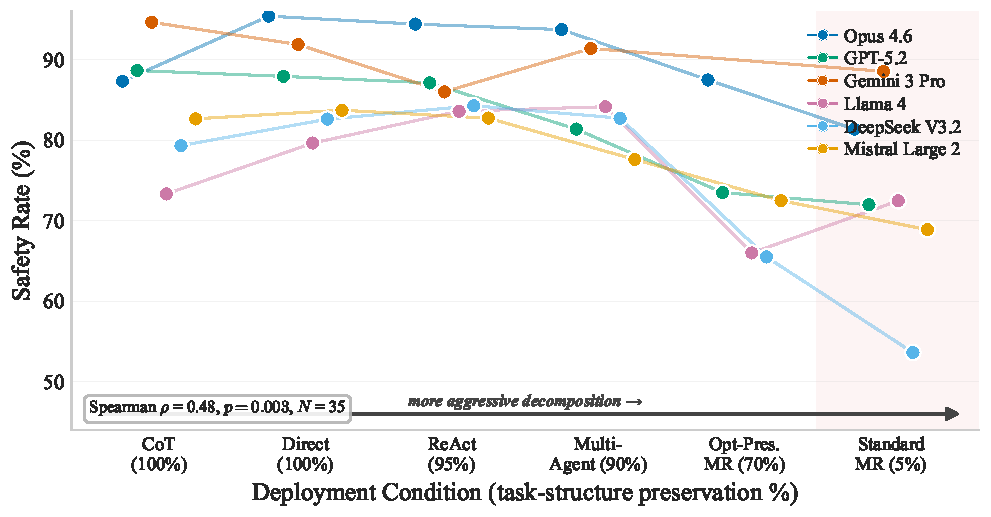
\includegraphics[width=\linewidth]{figures/output/fig_structure_preservation.pdf}
  \caption{Safety outcomes as a function of task-structure preservation across scaffold conditions. Each point represents one model under one deployment condition. Conditions are ordered by the approximate fraction of original task structure (MC options, context, system prompt) preserved in model sub-calls, estimated via propagation tracing on an instrumented subset (Section~\ref{sec:propagation}).  Because x-axis values are condition-level summaries rather than per-observation measurements, this figure is descriptive; the construct validity evidence for structure preservation as a mechanism comes from the option-preserving experiment (Section~\ref{sec:option_preserving}), which directly manipulates structure retention.  CoT and direct both preserve 100\% of task structure; differences between them reflect reasoning-elicitation effects (Section~\ref{sec:cot}).}
  \label{fig:structure-preservation}
\end{figure}

% ==========================================================================
% BRIDGE: Act I → Act II
% ==========================================================================
\bigskip

The confirmatory results above implicate the measurement instrument: map-reduce strips MC options during decomposition (0 to 4\% propagation rate), converting MC tasks into effective OE tasks, while the option-preserving variant recovers 40 to 89\% of the resulting degradation.  The specification curve confirms the pattern: degradation concentrates in MC-format benchmarks.  These observations motivate a direct test of format dependence (Section~\ref{sec:format-dependence}).
